	\section{Introduction}

\begin{frame}{introducing quantum communication}
Our model of quantum communication: Alice and Bob share an unlimited number of EPR pairs; have their own auxiliary quantum systems, and can communicate classical bits \footnote{Therefore they can do quantum teleportation.}. Cost of the communication protocol is the number of classical bits communicated. 

\begin{figure}[htbp]
	\centering % Centers the image
	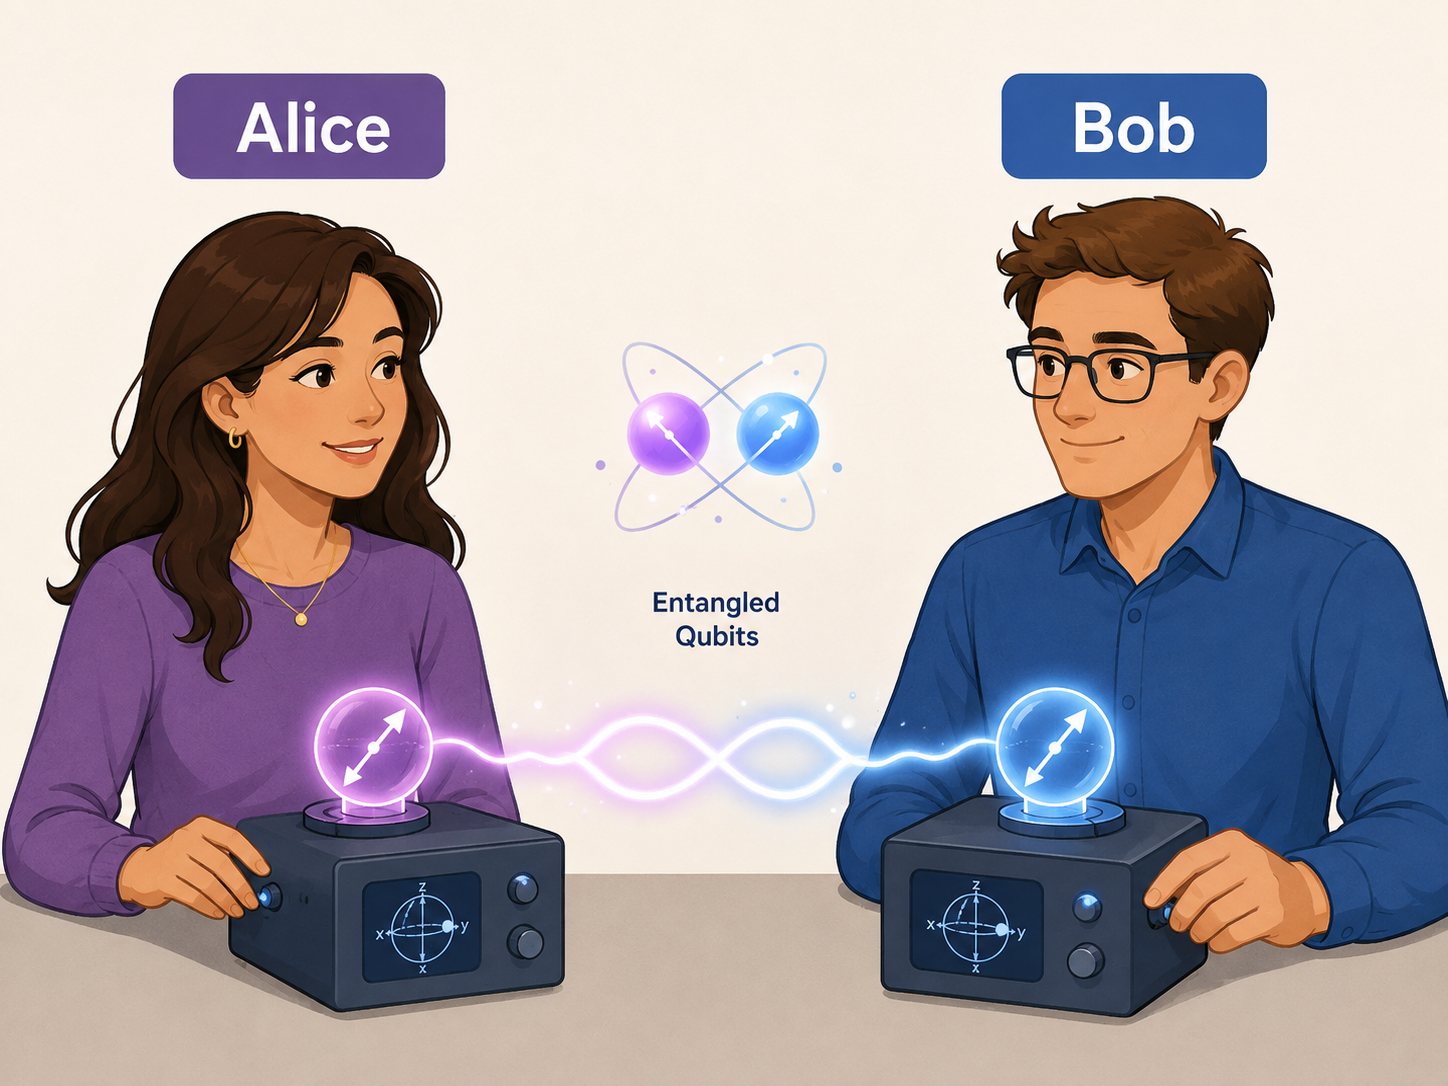
\includegraphics[width=0.7\textwidth]{quantum_communication.png} % Loads the image
	\caption{This is the caption for my image.}
	\label{fig:my_image} % Label used for cross-referencing
\end{figure}


\end{frame}	


\begin{frame}
	\textcolor{red}{\textbf{Quantum-Equivalence Conjecture}}: For a total function $f: \{0,1\}^n  \rightarrow \{0,1\}$, 
	$$R(f) \leq \text{poly}(Q(f))$$
	where
	\begin{itemize}
		\item $R(f)=$ classical randomized communication complexity
		\item $Q(f)=$ quantum communication complexity (with prior entanglement)
	\end{itemize}
	
	\textbf{Major open problem in communication complexity. First formally proposed by Shi and Zhu (2008)}
	
	
	
\end{frame}

\begin{frame}
	\textcolor{red}{\textbf{Our result}}: For AND functions, $f= g \circ \text{AND}_2$,
	$$ D(f) \leq \text{poly}(Q(f), \log(n)$$
	where $D(f)=$ classical deterministic communication complexity. \newline
	Thus, Quantum Equivalence Conjecture is true for AND functions up to $\text{polylog}(n)$ factors. \newline
	
	This answers an open problem of Razborov [2002].
	
	
	
\end{frame}

\begin{frame}
	
	\textbf{Why study AND functions?}
	\begin{itemize}
		\item<1-> Lifted functions form a large class of interesting communication problems. They form a testbed for all major conjectures in communication complexity (e.g, Log Rank Conjecture, Log Approximate Rank Conjecture [now known to be false], Quantum Equivalence Conjecture)
		\item<2-> Of particular interest is the case when the lifting gadget is as simple as possible, i.e., it has only two bits. In this case, the gadget does not have too much ability to obfuscate the inputs between Alice and Bob.
		\item<3-> There are only two nontrivial gadgets on 2 bits: XOR and AND. Both XOR and AND functions have been extensively studied in the literature.
	\end{itemize}
	
\end{frame}



\begin{frame}
	
	\textbf{AND functions}
	\begin{itemize}
		\item<1-> There is a base function $g: \{0,1\}^n \rightarrow \{0,1\}$. Alice has an input $x \in \{0,1\}^n$, Bob has an input $y \in \{0,1\}^n$. Their goal is to compute
		$$g(x_1 \land y_1, \cdots  , x_n \land y_n)$$
	\end{itemize}
	
\end{frame}



\begin{frame}{Prior work}
	\begin{itemize}
		\item<1-> \textbf{Razborov (2002)} proved the Equivalence conjecture for functions of the form $g \circ \text{AND}_2$, where $g$ is a symmetric function. 
		\item<2-> An easy adaptation of the same argument proves the results for functions of the form $g \circ h$, where $h$ is any gadget inside whose truth table both AND and OR can be embedded.
		\item<3-> \textbf{Burhman and deWolf (2003)} noticed a relation between $Q(g \circ \text{AND}_2)$ and various complexity measures of $g$, and conjectured a particular relation between them (to be described in detail soon).
		\item<4->\textbf{Kremer (1996)} proved log-approximate rank lower bounds quantum communication complexity.
		\item<5-> \textbf{Lovett, Knop, McGuire, Yuan (2021)} proved the log rank conjecture for AND functions. By an intermediate result in their proof, it became  clear that proving the relation conjectured by Burhman and deWolf would also imply the Quantum Equivalence Conjecture for $\text{AND}$ functions.
	\end{itemize}
	
\end{frame}



\begin{frame}{Prior work}
	\begin{itemize}
		\item<1-> \textbf{Chattopadhyay, Dahiya, Lovett (2026)} proved that de-Morgan sparsity and approximate de-Morgan sparsity are polynomially related.
		\item<2-> They also show the Quantum Equivalence Conjecture for functions of the form $g \circ \text{EQ}_4$.
		\item<3-> We extend their work to show the relation between quantities conjectured by Burhman and deWolf. This implies the Quantum-Equivalence Conjecture for AND functions.
	\end{itemize}
	
\end{frame}